\documentclass[11pt,a4paper]{article}

\usepackage{TypeBac}
\usepackage{listings}

\begin{document}
\input{\detokenize{/home/fenarius/Travail/Cours/Commun/latex/Macros.tex}}

\TBNSI{Février 2023}
\vspace{0.2cm}
\pythonmode



\Exo{Analyse et écriture de programmes récursifs}{\textit{2023 Sujet zéro \bac}}

\QListe
\item
\SQListe
\item Expliquer en quelques mots ce qu'est une fonction récursive
\item On considère la fonction Python suivante :
\begin{lstlisting}
def compte_rebours(n):
    """ n est un entier positif ou nul """
    if n >= 0:
        print(n)
        compte_rebours(n-1)
\end{lstlisting}
L'appel {\tt compte\_rebours(3)} affiche successivement les nombres 3, 2, 1 et 0. Expliquer pourquoi le programme s'arrête après l'affichage du nombre 0.
\FinListe
\item En mathématiques, la factorielle d'un entier naturel $n$ est le produit des nombres entiers strictement positifs inférieurs ou égaux à $n$. Par convention, la factorielle de 0 est 1. Par exemple :
\begin{itemize}
\item[\textbullet] la factorielle de 1 est 1
\item[\textbullet] la factorielle de 2 est $2\times 1 = 2$
\item[\textbullet] la factorielle de 3 est $3 \times 2 \times 1 = 6$
\item[\textbullet] la factorielle de 4 est $4\times 3 \times 2 \times 1 = 24$ \dots
\end{itemize}
Recopier et compléter sur votre copie le programme donné ci-dessous afin que la fonction récursive {\tt fact} renvoie la factorielle de l'entier passé en paramètre de cette fonction.

Exemple : {\tt fact(4)} renvoie {\tt 24}.
\begin{lstlisting}
def fact(n):
    """ Renvoie le produit des nombres entiers strictement positifs inférieurs à n """
    if n == 0:
        return .........
    else:
        return .........
\end{lstlisting}
\item La fonction {\tt somme\_entiers\_rec} ci-dessous permet de calculer la somme des entiers, de 0 à l'entier naturel $n$ passé en paramètre.

Par exemple :
\begin{itemize}
    \item[\textbullet] pour {\tt n} = 0, la fonction renvoie la valeur  0
    \item[\textbullet] pour {\tt n} = 1, la fonction renvoie la valeur  $0 + 1 = 1$.
    \item[] \dots
    \item[\textbullet]  pour {\tt n} = 4, la fonction renvoie la valeur $0 + 1 + 2 + 3 + 4 = 10$.
\end{itemize}
\begin{lstlisting}
def somme_entiers_rec(n):
    """ Permet de calculer la somme des entiers, de 0 à l'entier naturel n """
    if n == 0:
        return 0
    else:
        print(n) #pour vérification
        return n + somme_entiers_rec(n - 1)
\end{lstlisting}
L'instruction {\tt print(n)} de la ligne 6 dans le code précédent a été insérée afin de mettre en évidence le mécanisme en oeuvre au niveau des appels récursifs.
\SQListe
\item Ecrire ce qui sera affiché dans la console après l'exécution de la ligne suivante : \\
{\tt res = somme\_entiers\_rec(3)}
\item Quelle valeur sera alors affectée à la variable {\tt res} ?
\FinListe
\item Ecrire en Python une fonction {\tt somme\_entiers} non récursive : cette fonction devra prendre en argument un entier naturel $n$ et renvoyer la somme des entiers de 0 à $n$ compris. Elle devra donc renvoyer le même résultat que la fonction {\tt somme\_entiers\_rec} définie à la question {\bf 3}.

Exemple : {\tt somme\_entiers(4)} renvoie 10.
\FinListe

\separateur



\Exo{Programmation objet en langage Python}{\textit{2022 Asie-Pacifique \bac}}

Un fabricant de brioches décide d’informatiser sa gestion des stocks. Il écrit pour cela un programme en langage Python. Une partie de son travail consiste à développer une classe Stock dont la première version est la suivante :

\begin{lstlisting}
class Stock:
    def __init__(self):
        self.qt_farine = 0  # quantité de farine initialisée à 0 g
        self.nb_oeufs = 0   # quantité de d'oeufs (0 à l'initialisation)
        self.qt_beurre = 0  # quantité de beurre initialisée à 0 g
\end{lstlisting}

\QListe
\item Ecrire une méthode {\tt ajouter\_beurre(self,qt) qui ajoute la quantité {\tt qt} de beurre  un objet de la classe {\tt Stock}} \\

\parindent -1cm 
\parbox{\textwidth}{On admet que l'on a écrit deux autres méthodes {\tt ajouter\_farine} et {\tt ajouter\_oeufs} qui ont des fonctionnements analogues.} \vspace{0.2cm}


\item Ecrire une méthode {\tt afficher(self)} qui affiche la quantité de farine, d'oeufs et de beurre d'un objet de type {\tt Stock}. L'exemple ci-dessous illustre l'exécution de cette méthode dans la console :
\begin{lstlisting}
>>> mon_stock = Stock()
>>> mon_stock.afficher()
farine: 0
oeuf: 0
beurre: 0
>>> mon_stock.ajouter_beurre(560)
>>> mon_stock.afficher()
farine: 0
oeuf: 0
beurre: 560
\end{lstlisting}

\item Pour faire une brioche, il faut 350 g de farine, 175 g de beurre et 4 oeufs. Ecrire une méthode {\tt stock\_suffisant\_brioche(self)} qui renvoie un booléen : {\tt True} s'il y a assez d'ingrédients dans le stock pour faire une brioche et {\tt False} sinon.
\item On considère la méthode supplémentaire {\tt produire(self)} de la classe {\tt Stock} donnée par le code suivant :
\begin{lstlisting}
def produire(self)
    res = 0
    while self.stock_suffisant_brioche():
        self.qt_beurre = self.qt_beurre - 175
        self.qt_farine = self.qt_farine - 350
        self.nb_oeufs = self.nb_oeufs -4
        res = res + 1
    return res
\end{lstlisting}

On considère une stock défini par les instructions suivantes :
\begin{lstlisting}
>>> mon_stock = Stock()
>>> mon_stock.ajouter_beurre(1000)
>>> mon_stock.ajouter_farine(1000)
>>> mon_stock.ajouter_oeufs(10)
\end{lstlisting}
\SQListe
\item On exécute ensuite l'instruction 
\begin{lstlisting}
>>> mon_stock.produire()
\end{lstlisting}
Quelle valeur s'affiche dans la console ? Que représente cette valeur ?
\item On exécute ensuite l'instruction
\begin{lstlisting}
>>> mon_stock.afficher()
\end{lstlisting}
Que s'affiche-t-il dans la console ?
\FinListe
\item L'industriel possède $n$ lieux de production distincts et donc $n$ stocks distincts. On suppose que ces stocks sont dans une liste dont chaque élément est une objet de type {\tt Stock}. Ecrire une fonction Python {\tt nb\_brioches} prenant pour seul paramètre une liste de d'objets de type {\tt Stock} et renvoie le nombre total de brioches produites.
\FinListe

\separateur

\Exo{Structure de données (piles) -- Base de données}{\textit{Etranger 2021} \bac}

Cette exercice se compose de deux parties \textbf{indépendantes}.

\vspace{0.2cm}
\large{\bf  Partie A}

Dans cet exercice, on considère une pile d'entiers positifs. On suppose que les autre fonctions suivantes ont été programmées préalablement en Python :
\begin{itemize}
    \item {\tt empiler(P,e)} : ajoute l'élément {\tt e} sur la pile {\tt P};
    \item {\tt depiler(P)} : enlève le sommet de la pile {\tt P} et renvoie la valeur de ce sommet
    \item {\tt est\_vide(P)} : renvoie {\tt True} si la pile est vide et {\tt False} sinon ;
    \item {\tt creer\_pile()} : retourne une pile vide.
\end{itemize}

\textbf{Dans cet exercice, seule l'utilisation de ces quatre fonctions sur la structure de données pile est autorisée}

\QListe
\item \textbf{Recopier} le schéma ci-dessous et le compléter sur votre copie en exécutant les appels de fonctions donnés. On écrira ce que renvoie la fonction utilisé dans chaque cas, et on indiquera {\tt None} si la fonction ne renvoie aucune valeur :

\begin{tabularx}{\linewidth}{|Y|Y|Y|Y|Y|}
\hline
Etapes  & Etape 0 \newline Pile d'origine {\tt P} & Etape 1  \newline {\tt empiler(P,8)} & Etape 2 \newline {\tt depiler(P)} & Etape 3 \newline {\tt est\_vide(P)} \\
\hline
Pile &  \  \newline 
 \begin{tabular}{|c|} 
     \\
    \hline
    \ 4 \ \\
    \hline
    7 \\
    \hline
    1 \\
    \hline
    5 \\
    \hline
 \end{tabular} \ \newline
 & 
 \  \newline 
 \begin{tabular}{|c|} 
    \dots \\
    \hline
    \dots \\
    \hline
    \dots \\
    \hline
    \dots \\
    \hline
    \dots \\
    \hline
 \end{tabular} \ \newline
 & 
 \  \newline 
 \begin{tabular}{|c|} 
    \dots \\
    \hline
    \dots \\
    \hline
    \dots \\
    \hline
    \dots \\
    \hline
    \dots \\
    \hline
 \end{tabular} \ \newline
 & 
 \  \newline 
 \begin{tabular}{|c|} 
    \dots \\
    \hline
    \dots \\
    \hline
    \dots \\
    \hline
    \dots \\
    \hline
    \dots \\
    \hline
 \end{tabular} \ \newline
 \\ 
 \hline 
 \multicolumn{2}{|c|}{Valeurs renvoyées}   & \dots & \dots & \dots \\
 \hline 
\end{tabularx}
\item On propose la fonction ci-dessous, qui prend en argument une pile {\tt P} et renvoie un couple de piles :
\begin{lstlisting}
def transforme(P):
    Q = creer_pile()
    while not est_vide(P) :
        v = depile(P)
        empile(Q,v)
    return (P,Q)
\end{lstlisting}
\textbf{Recopier et compléter} sur votre copie le document ci-dessous :
\begin{center}
    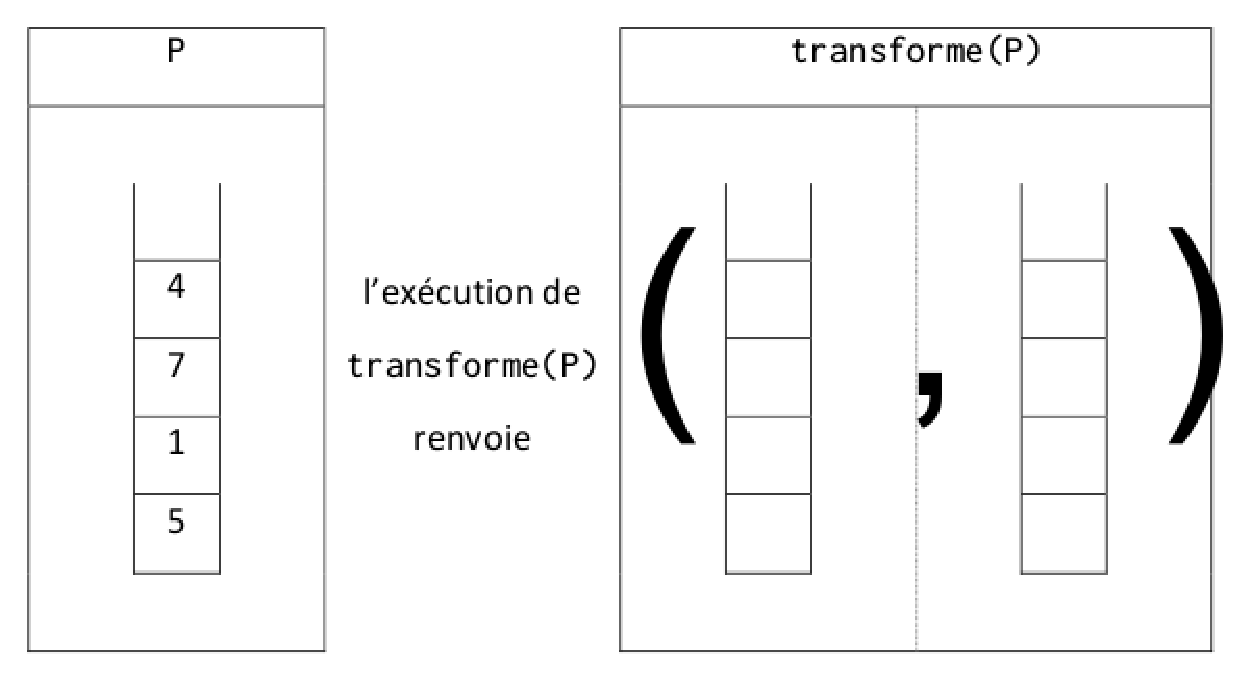
\includegraphics[width=300px]{TypeBac1-a.eps}
\end{center}
\item \textbf{Ecrire} une fonction en langage Python {\tt maximum(P)} recevant une pile {\tt P} comme argument et qui renvoie la valeur maximale de cette pile. On ne s'interdit pas qu'après exécution de la fonction, la pile soit vide.
\FinListe

\vspace{0.2cm}
\large{\bf  Partie B}

On suppose qu'on dispose d'une base de données des processus lancés sur un ordinateur à un instant donné. Cette base de données est constituée d'une seule table appelée {\tt processus} et contenant les champs suivants :
\begin{itemize}
    \item {\tt pid} : le {\sc pid} du processus
    \item {\tt ppid}: le {\sc ppid} du processus
    \item {\tt user}: le nom du propriétaire du processus
    \item {\tt time}: le temps d'exécution du processus (en secondes)
\end{itemize}

\QListe
\item A propos des processus
\SQListe
\item Rappeler rapidement ce qu'est le {\tt pid} d'un processus
\item Parmi les commandes suivantes, indiquer sur votre copie laquelle permet de tuer un processus en cours d'exécution.
    \begin{itemize}
        \item {\tt delete}
        \item {\tt stop}
        \item {\tt remove}
        \item {\tt end}
        \item {\tt kill}
        \item {\tt interrupt}
    \end{itemize}
\item Expliquer pourquoi {\tt pid} peut être utilisé comme clé primaire de cette table et pas {\tt user}
\FinListe
\item Quelques requêtes
\SQListe
\item Ecrire une requête {\sc sql} permettant d'afficher les champs {\tt pid} et {\tt user}.
\item Ecrire une requête {\sc sql} permettant d'afficher les processus de l'utilisateur {\tt root}.
\item Ecrire une requête {\sc sql} permettant d'afficher tous les fils du processus de {\tt pid} 712.
\item Ecrire une requête {\sc sql} permettant d'afficher les {\tt pid} des processus ayant un temps d'exécution supérieur à 50 secondes.
\item Ecrire une requête {\sc sql} permettant d'afficher les processus classés dans l'ordre alphabétique du propriétaire du processus.
\item Ecrire une requête {\sc sql} permettant d'afficher les 5 processus ayant le plus long temps d'exécution.
\FinListe
\FinListe


\end{document}

